\chapter{METODOLOGI PENELITIAN}
Metodologi penelitian menggambarkan urutan langkah pelaksanaan penelitian atau strategi peneliti, rencana, tempat, waktu, pengambilan data dalam menjawab masalah penelitian. Pada bagian ini diuraikan metode yang digunakan secara rinci. Dengan demikian dapat diperkirakan hasil penelitian yang akan diperoleh secara utuh. Dalam bagian metodologi penelitian perlu diuraikan beberapa hal berikut:

\section{Data dan Pengumpulan Data}
Pengumpulan data akan dilakukan dengan cara observasi dan wawancara kepada pihak sekolah SMK NEGERI 1 KARANG BARU untuk mencapai tujuan penelitian.

\section{Rancangan Sistem}
Rancangan system terdiri dari tahapan dalam bentuk blok diagram.

\subsection{Rancangan Use Case Diagram}

Ada 2 aktor dalam \emph{use case diagram} yaitu \emph{user} dan \emph{admin}, masing - masing memiliki peran penting dalam aplikasi, \emph{user} dapat menggunakan aplikasi mulai dari \emph{login}, melihat profil, melihat daftar pelajaran, daftar siswa, melakukan penjadwalan absensi, dan \emph{logout}. Selanjutnya \emph{admin} melakukan \emph{maintenance} seperti mengelola data guru dan siswa, serta mengubah mata pelajaran pada aplikasi. Berikut \emph{use case diagram} pada aplikasi absensi dapat dilihat pada gambar \ref{lab:use}.

\begin{figure}[h]
\centering
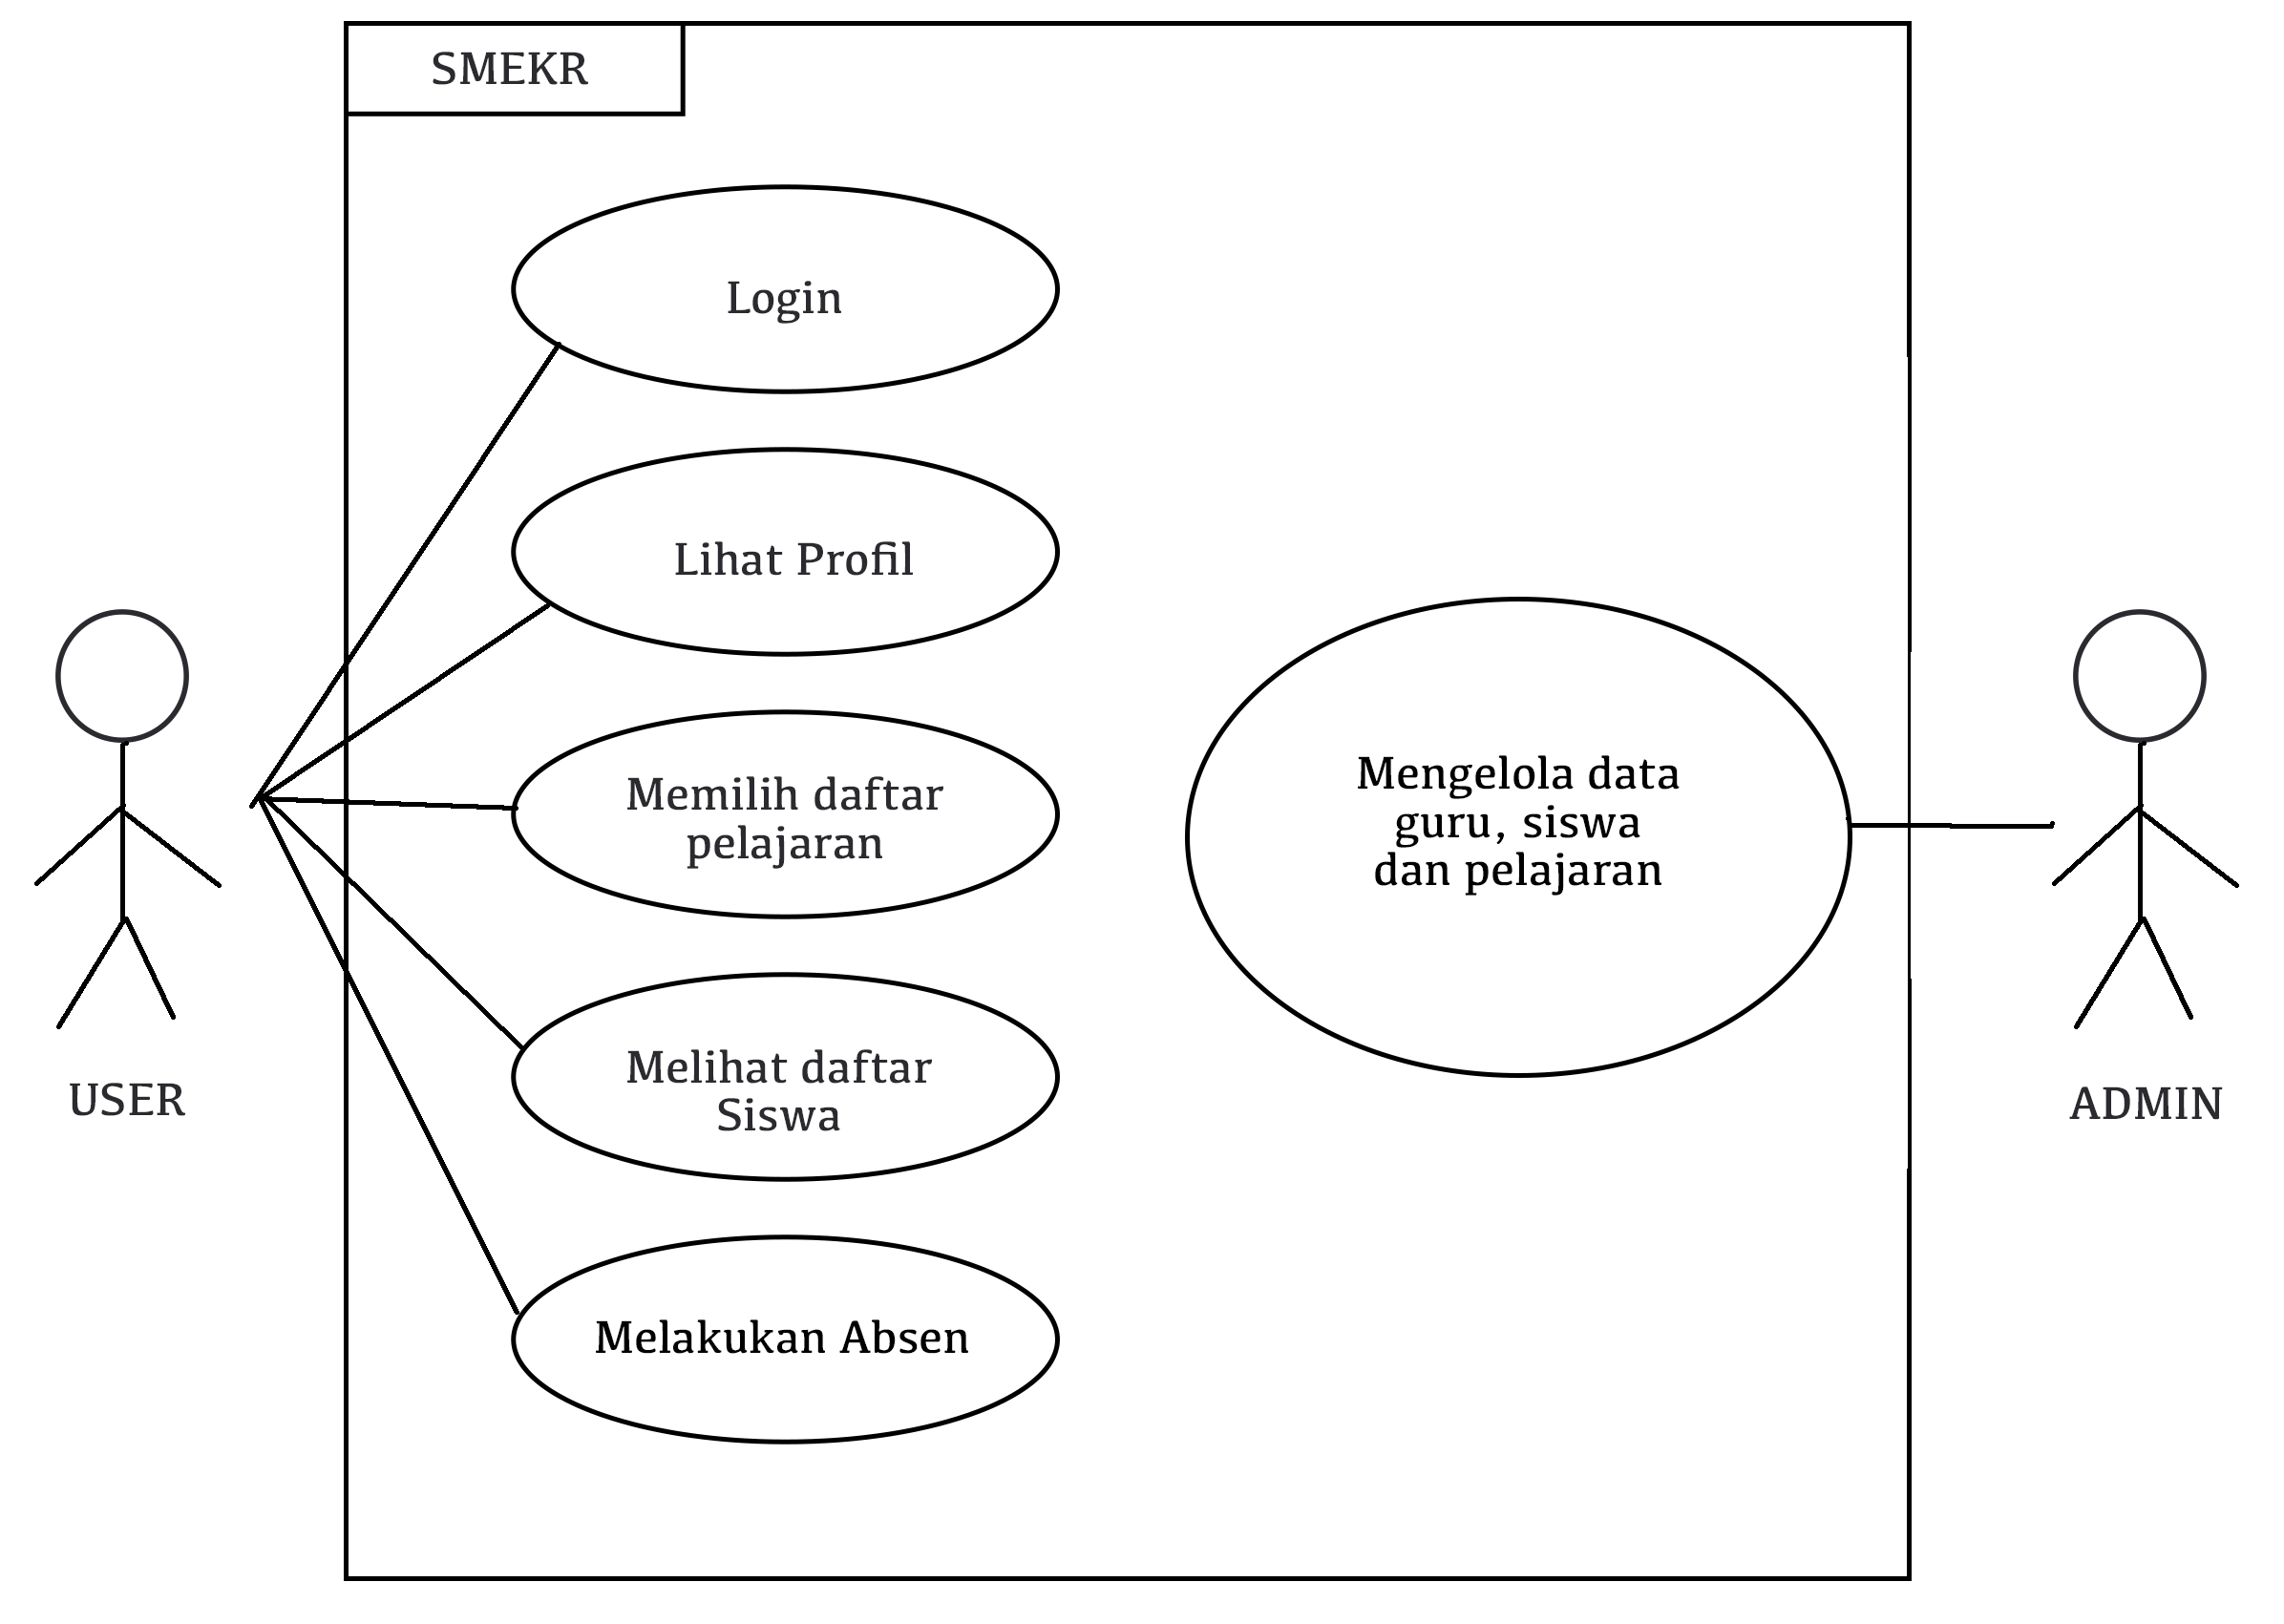
\includegraphics[width=9cm]{ussd}
\caption{Gambar Use Case Diagram}
\label{lab:use}
\end{figure}


\subsection{Diagram Activity}
Pada alur selanjutnya menjelaskan aktifitas alur \emph{user} dan sistem. Gambar \ref{lab:login}. menunjukan diagram \emph{activity} aplikasi.

\begin{figure}[h]
\centering
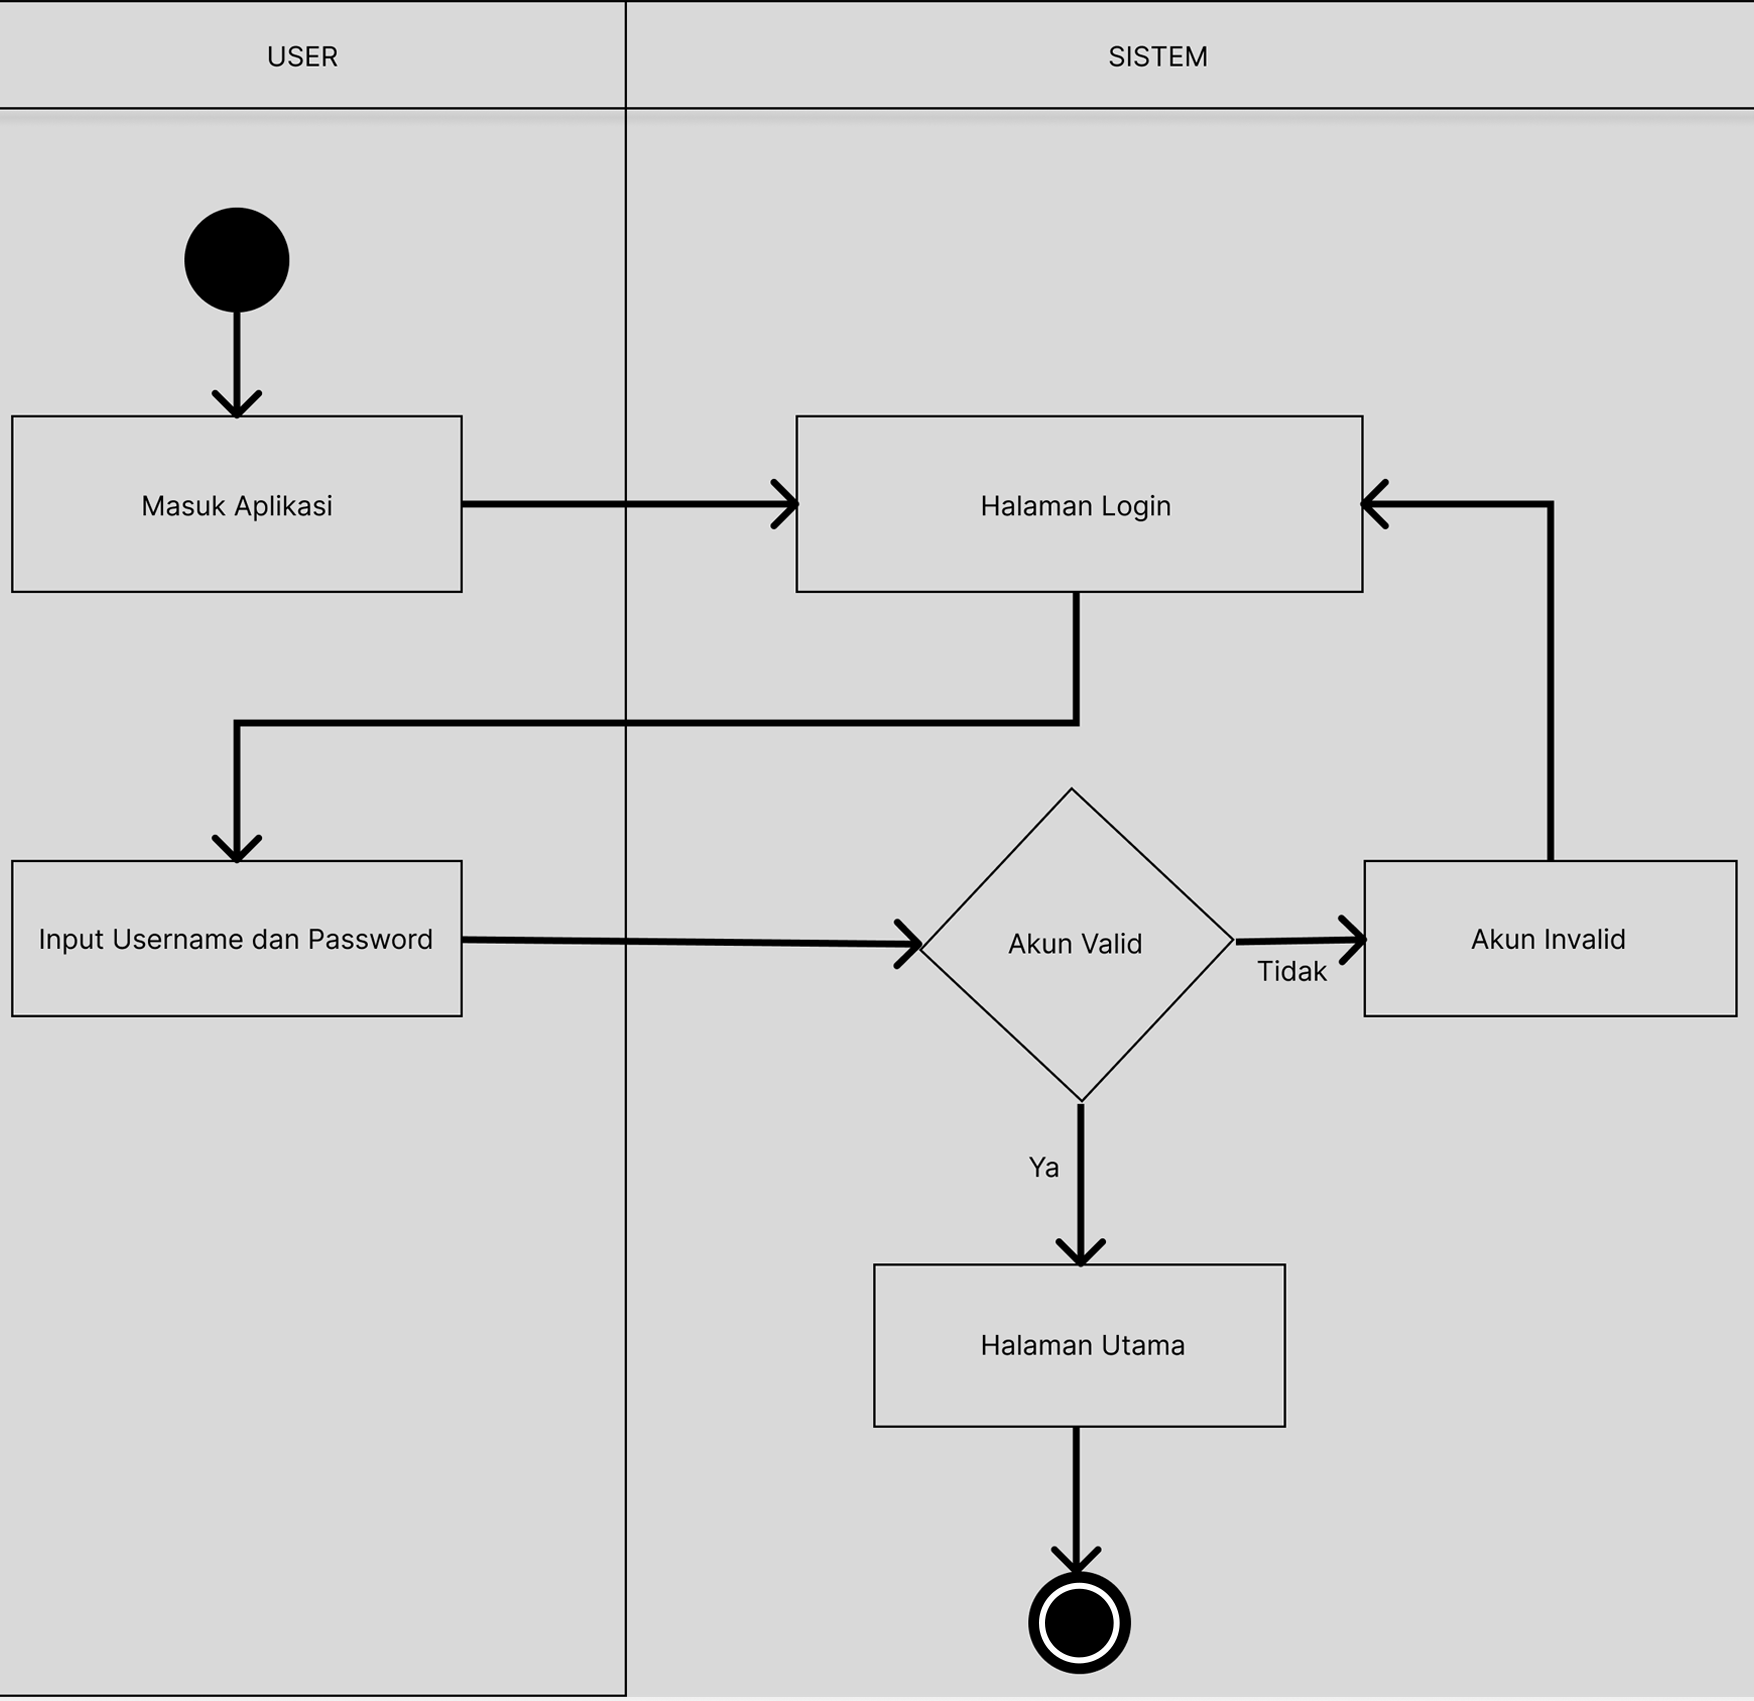
\includegraphics[width=14cm]{LOGIIN}
\caption{Gambar Diagram Activity Login}
\label{lab:login}
\end{figure}\
Pada gambar diatas menjelaskan proses \emph{login user} saat masuk ke dalam aplikasi, selanjutnya sistem menampilkan halaman \emph{login} dan \emph{user} memasukan \emph{username} dan \emph{password} yang sudah ditentukan oleh admin.
\newpage

\begin{figure}[h]
\centering
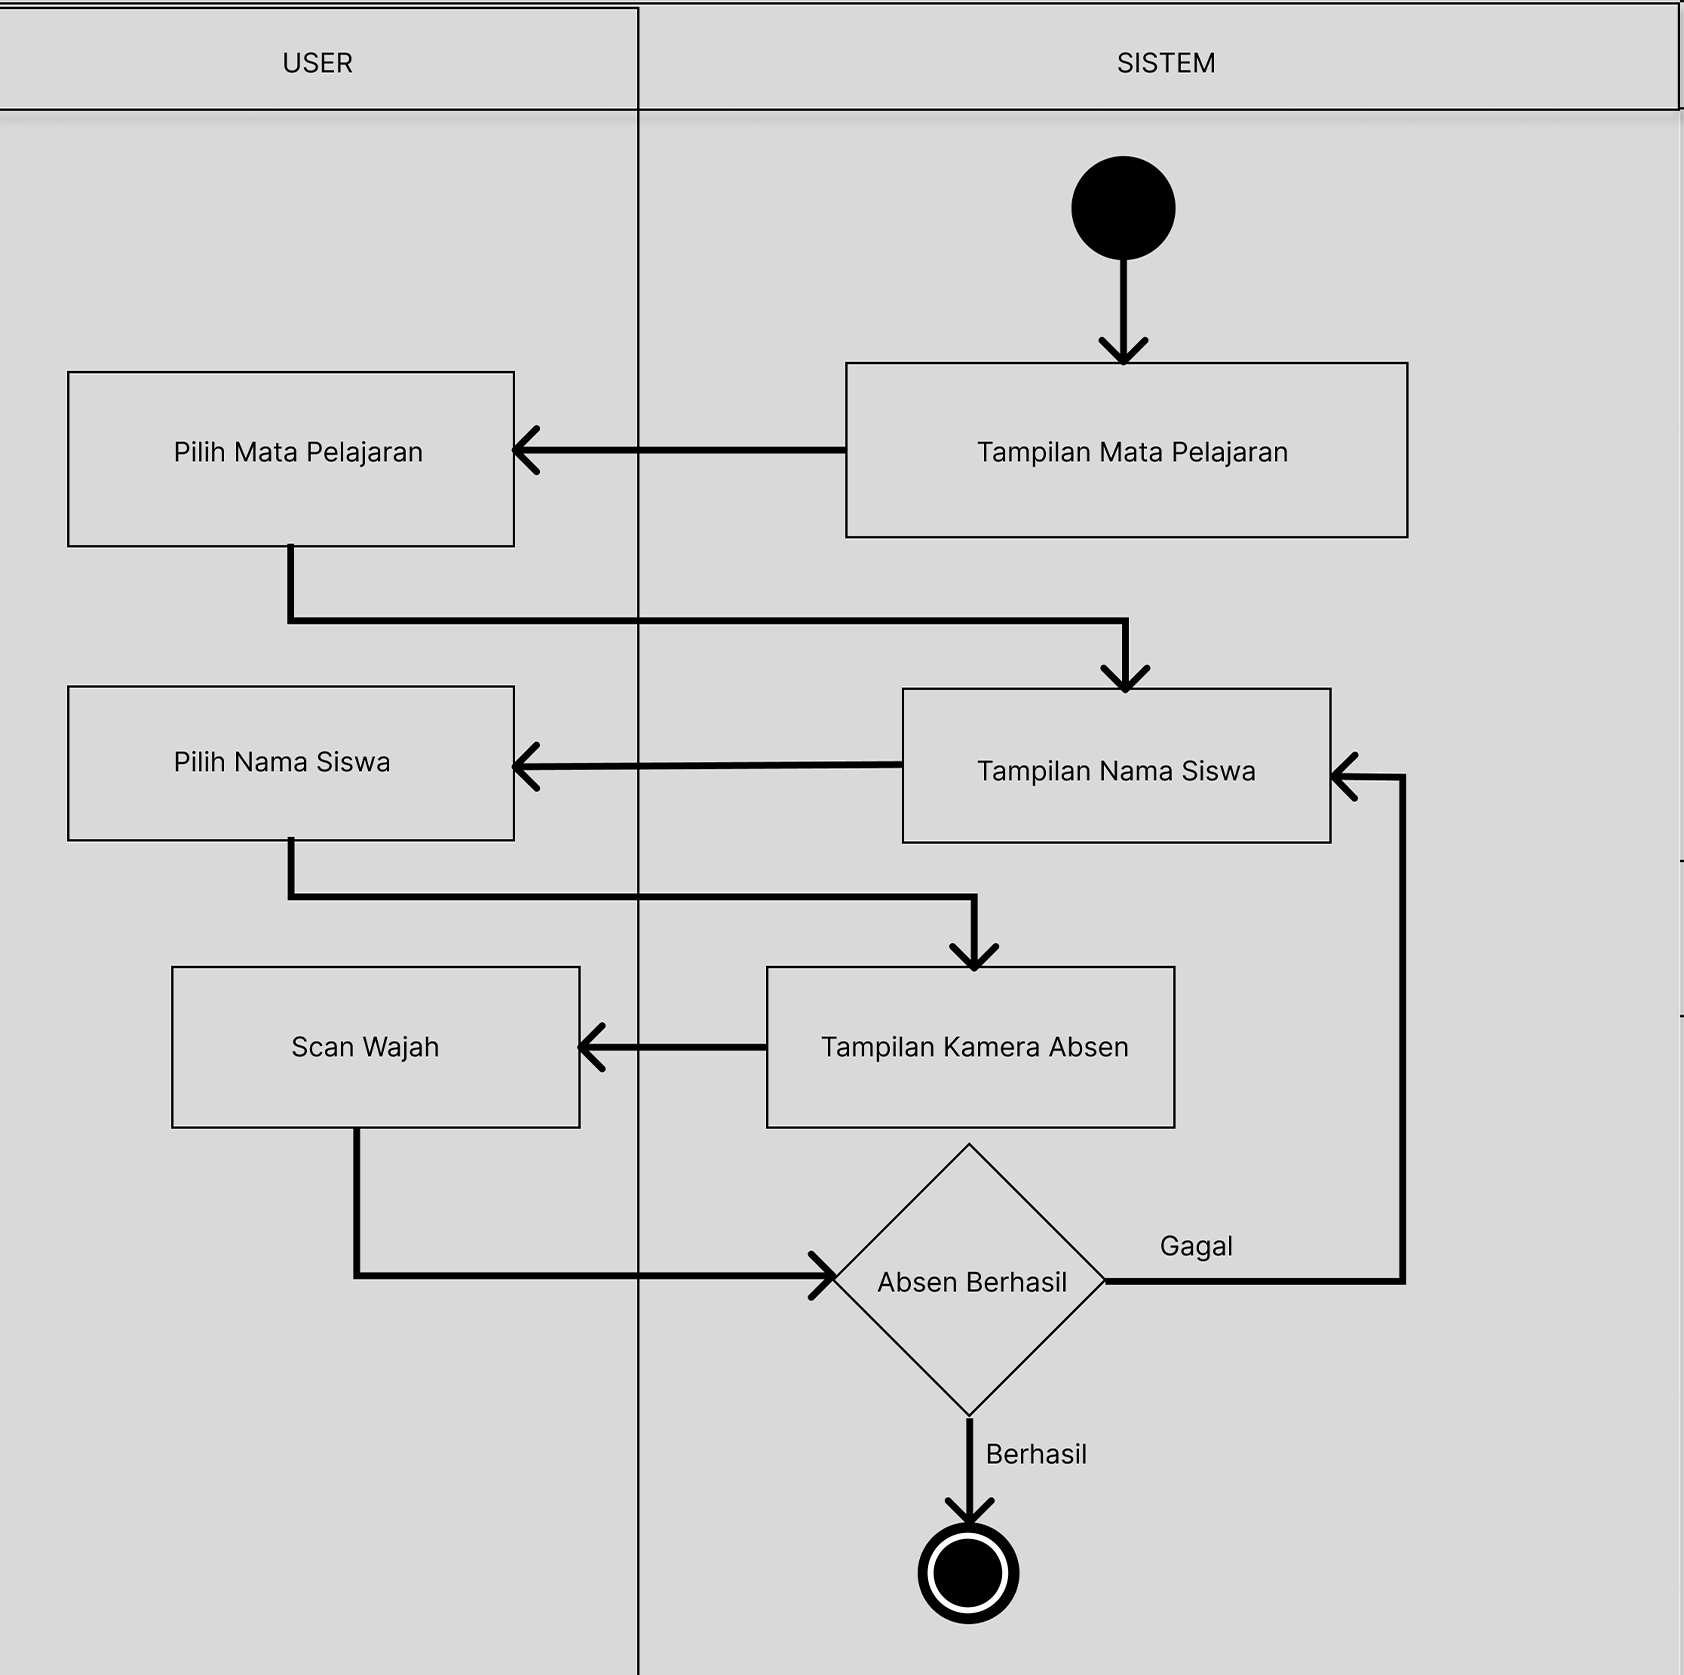
\includegraphics[width=14cm]{absen}
\caption{Gambar Diagram Activity Absen}
\label{lab:absen}
\end{figure}\
Pada gambar \ref{lab:absen} diatas menjelaskan proses presensi yang dilakukan \emph{user}, kemudian sistem menampilkan daftar siswa, \emph{user} melakukan \emph{scanning} wajah pada aplikasi, jika wajah sudah terdata maka presensi berhasil, jika tidak berhasil akan diarahkan oleh sistem untuk melakukan pemilihan ulang daftar siswa.
\newpage

\begin{figure}[h]
\centering
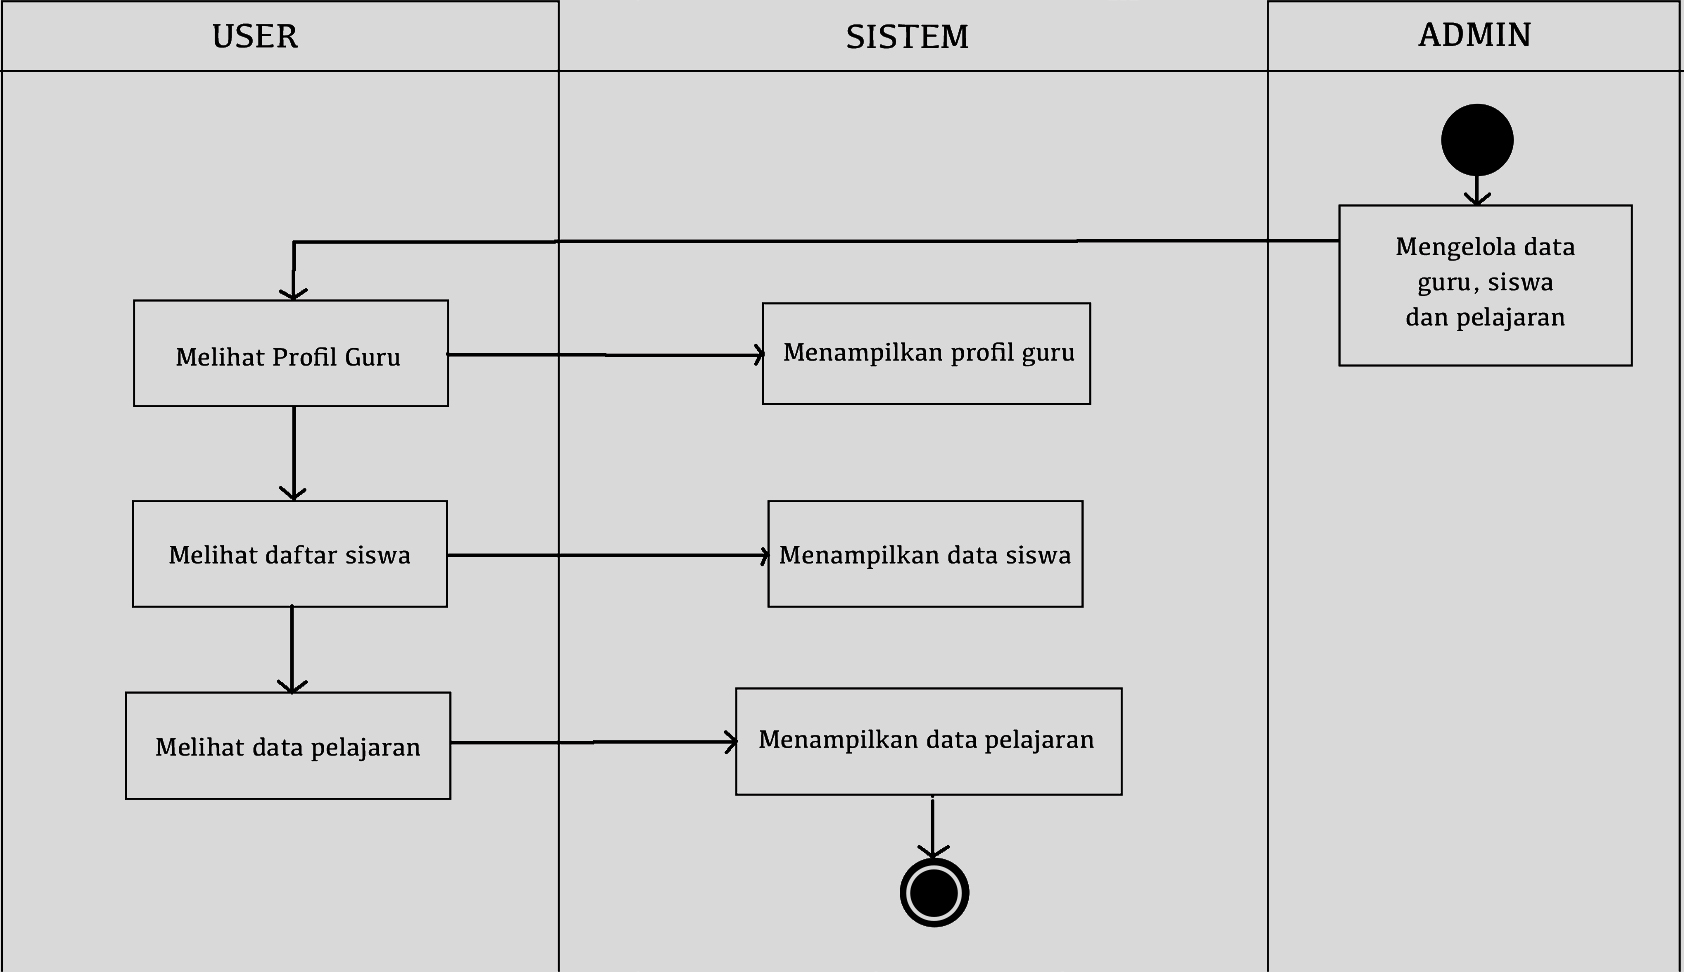
\includegraphics[width=14cm]{data}
\caption{Gambar Diagram Activity Data}
\label{lab:data}
\end{figure}\
Pada gambar \ref{lab:data}. diatas menjelaskan proses admin melakukan penambahan data, kemudian \emph{user} dapat melihat data yang telah diubah yang ditampilkan oleh sistem.
\newpage

\section{Metode Penelitian}
\subsection{Metodologi Penelitian}
Metodologi penelitian dapat dilihat pada gambar dibawah ini.
\begin{figure}[h]
\centering
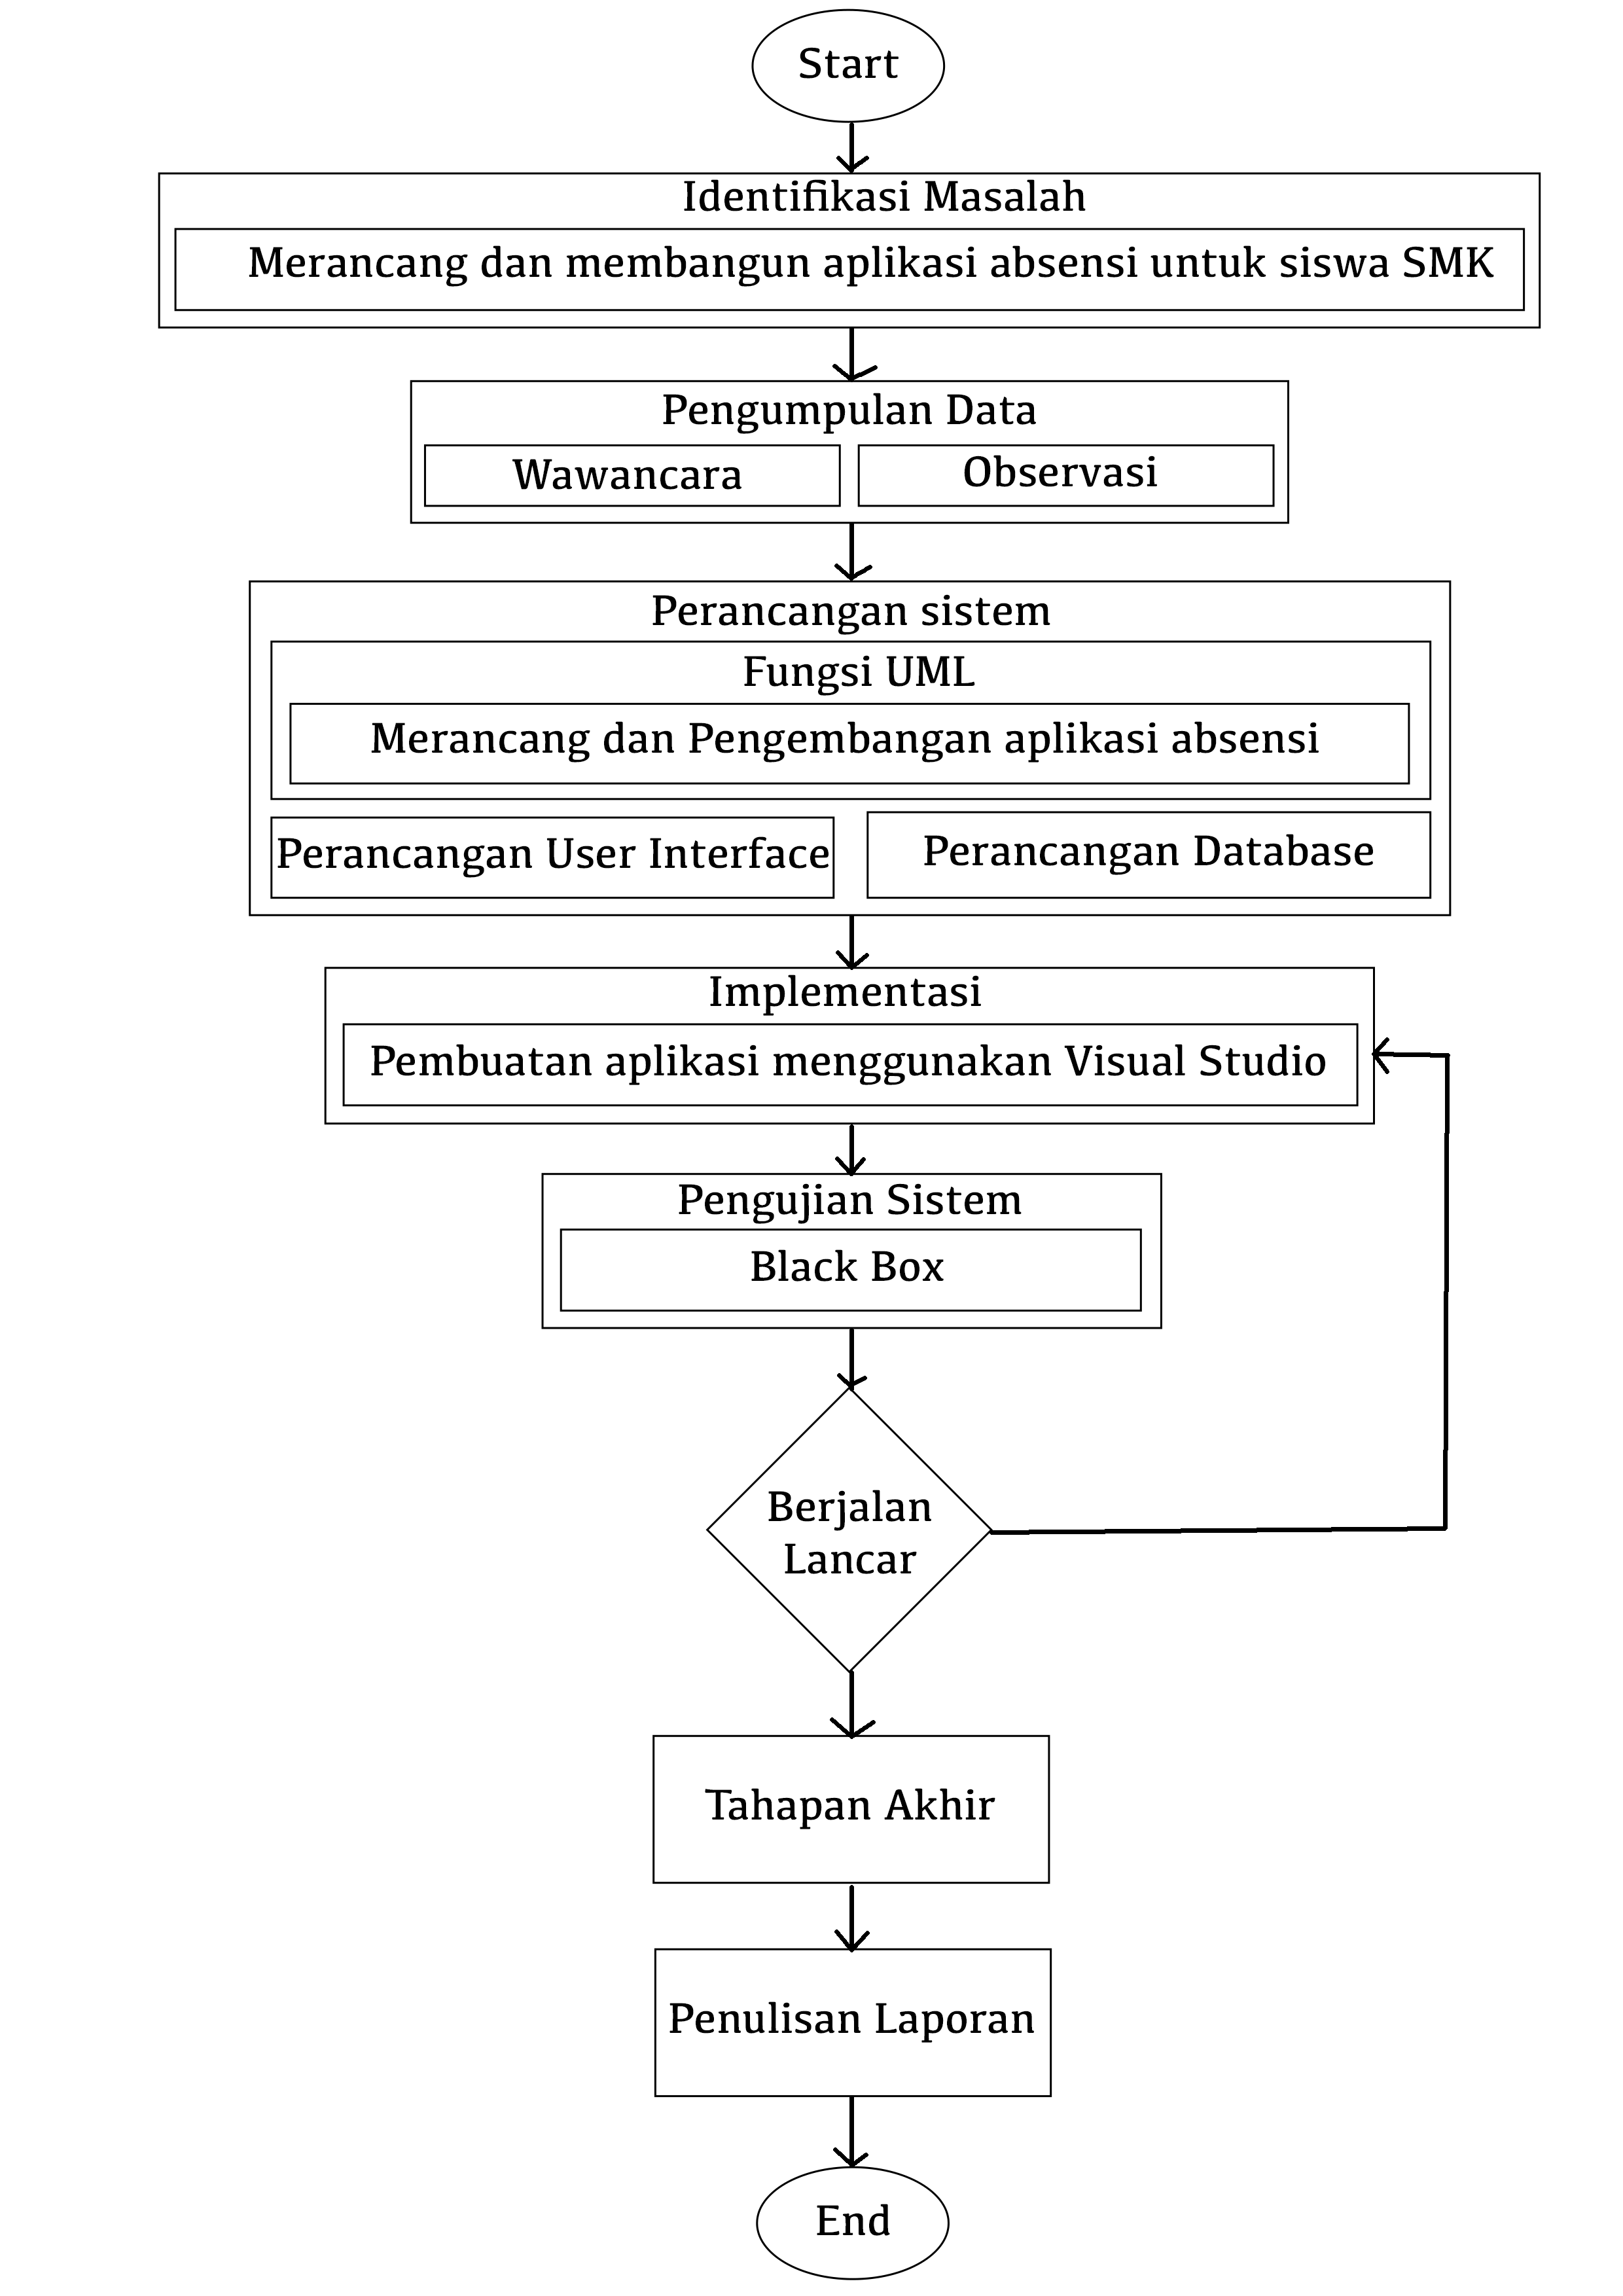
\includegraphics[width=11cm]{met}
\caption{Gambar Metodologi Penelitian}
\label{lab:met}
\end{figure}\
\newpage

\subsection{Perancangan Sistem}
Sistem yang digunakan berupa membaca struktur wajah saat melakukan absen, sistem presensi hanya berlaku didalam kelas menggunakan Smartphone guru.
\begin{enumerate}
\item Fungsional UML\\
Penulis merancang UML diagram, yaitu \emph{Use Case Diagram}
\item Perancangan \emph{User-Interface}\\
Menu yang ada didalam apliaksi meliputi, Login, presensi, data siswa, dan data mata pelajaran.
\item Perancangan \emph{Database}\\
Perancangan database berfungsi untuk menyimpan data siswa.
\end{enumerate} 

\subsection{Implementasi}
Perancangan yang sudah dibuat  di implementasikan menggunakan aplikasi visual studio hingga menjadi aplikasi presensi.

\section{Teknik Pengujian}
Tahapan pengujian dilakukan menggunakan \emph{black box} untuk menguji kelayakan aplikasi dan melihat terjadinya error menggunakan teknik \emph{Equivalence Partitioning} yaitu teknik yang bekerja dengan cara membagi data input dari beberapa perangkat lunak menjadi beberapa partisi data yang dibagi menjadi beberapa domain ke pengguna. Berikut contoh tabel pengujian \emph{black box}.


\section{Hasil yang diharapkan}
Dengan demikian, hasil yang diharapkan yaitu terciptanya aplikasi presensi dengan \emph{Face Recognition} yang akan mempermudah sistem presensi di SMK NEGERI 1 KARANG BARU.
